\section{Overview}

The proposed methodology transforms source files into source code minimaps and
uses these minimaps as visual signatures for software analysis. The method is
organized as a pipeline with seven stages:

\begin{enumerate}
    \item repository selection and file discovery;
    \item filtering of source and auxiliary artifacts;
    \item anonymization of lexical content;
    \item minimap rendering;
    \item catalog construction;
    \item model training and evaluation;
    \item interpretation and tool integration.
\end{enumerate}

Figure~\ref{fig:workflow} presents the general workflow adopted in the large-scale
study and reused as the methodological basis of this doctoral project.

\begin{figure}[ht]
    \centering
    \caption{General workflow for source code minimap analysis.}
    \label{fig:workflow}
    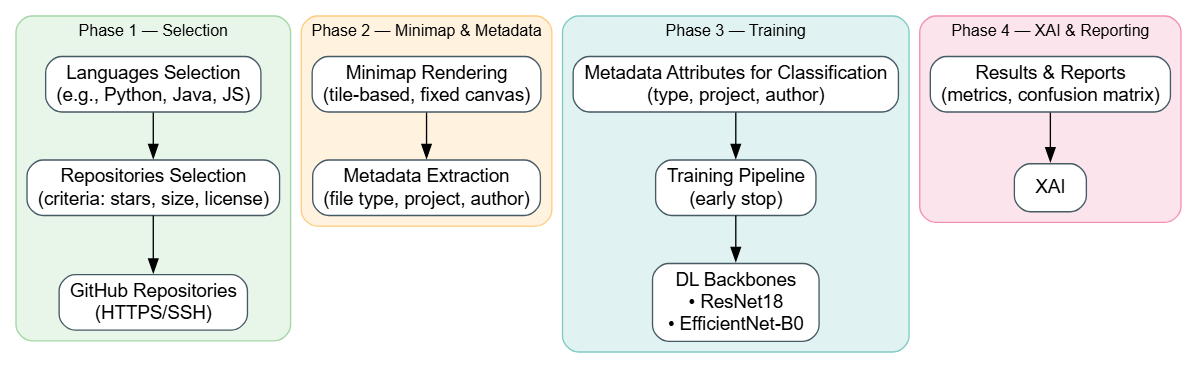
\includegraphics[width=0.95\textwidth]{figuras/workflow.png}
    \fautor
\end{figure}

The pipeline is intentionally modular. Minimap generation can be executed
without model training; anonymization can be strengthened or replaced; the same
catalog can support different objectives; and the trained models can be used
either in offline experiments or in IDE-integrated inference. This modularity is
important because the doctoral project combines empirical research, dataset
construction, explainability, and tool support.

\section{Repository Selection and File Discovery}

The repository-selection strategy depends on the research objective. For the
large-scale study, repositories were selected to cover multiple programming
languages and project conventions. The resulting corpus contains 100 open-source
projects across 10 languages \cite{gebara2025ciarp}. For future quality-related
studies, the selection must be refined to include repositories with known
quality indicators, code-smell labels, architectural roles, or defect history.

File discovery starts with recursive traversal of each repository. The traversal
records the relative path, file extension, size, and repository identifier. It
also applies exclusion rules to avoid files that would distort the dataset or
introduce redundant information. Typical exclusions include version-control
metadata, dependency folders, build outputs, binaries, vendored libraries, and
generated distribution folders such as \texttt{node\_modules}, \texttt{dist},
\texttt{build}, and \texttt{target}.

The filtering strategy must balance coverage and noise. If filtering is too
strict, the dataset may lose relevant software artifacts such as configuration
files, templates, and markup. If filtering is too permissive, the dataset may be
dominated by generated files, vendored code, or non-source artifacts. Because
minimaps can represent heterogeneous file types, the project does not restrict
the corpus to one programming language. Instead, file types are included when
they are meaningful for software analysis and when their role can be documented
in the catalog.

\section{Minimap Generation}

A source code minimap is generated by mapping the characters of a source file to
pixel intensities. The simplest form treats each character position as a visual
unit and each line as a row. The resulting image preserves aspects such as line
length, indentation, blank lines, punctuation density, and repeated structures.
Figure~\ref{fig:minimap-generation} illustrates the transformation from source
code to minimap.

\begin{figure}[ht]
    \centering
    \caption{Transformation of source code into a minimap representation.}
    \label{fig:minimap-generation}
    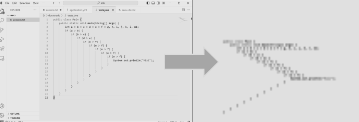
\includegraphics[width=0.88\textwidth]{figuras/minimap-generation.png}
    \fautor
\end{figure}

Two rendering strategies are considered:

\begin{description}
    \item[Variable-size minimaps.] The image width follows the length of the
    longest line, and the height follows the number of lines in the file. This
    representation preserves more information from the original artifact, but it
    produces images of different dimensions.

    \item[Fixed-size minimaps.] Each file is rendered or resized to a standard
    dimension, such as 128 by 128 pixels. This representation simplifies deep
    learning pipelines because all inputs share the same shape.
\end{description}

Figure~\ref{fig:fixed-variable} contrasts fixed-size and variable-size minimaps.
The first study evaluated both alternatives with handcrafted texture
descriptors, while the large-scale study adopted fixed 128 by 128 minimaps for
compatibility with convolutional backbones \cite{gebara2025iwssip,gebara2025ciarp}.

\begin{figure}[ht]
    \centering
    \caption{Comparison between variable-size and fixed-size minimaps.}
    \label{fig:fixed-variable}
    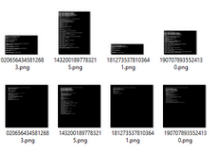
\includegraphics[width=0.82\textwidth]{figuras/fixed-variable-minimaps.png}
    \fautor
\end{figure}

Algorithm~\ref{alg:minimap-generation} summarizes the minimap generation
procedure in abstract form.

\begin{algorithm}[ht]
\caption{Source code minimap generation}
\label{alg:minimap-generation}
\begin{algorithmic}[1]
\Require Repository path $R$, file filters $F$, anonymization function $A$, target size $S$
\Ensure Minimap image set $M$ and metadata catalog $C$
\State $M \gets \emptyset$; $C \gets \emptyset$
\ForAll{file $f$ discovered recursively in $R$}
    \If{$f$ satisfies filters $F$}
        \State $content \gets$ read textual content from $f$
        \State $content' \gets A(content)$
        \State $image \gets$ render characters of $content'$ as pixel intensities
        \If{fixed-size mode is enabled}
            \State $image \gets$ resize or pad $image$ to target size $S$
        \EndIf
        \State $id \gets$ compute stable artifact identifier
        \State Add $(id, image)$ to $M$
        \State Add metadata for $f$ to $C$
    \EndIf
\EndFor
\State \Return $M, C$
\end{algorithmic}
\end{algorithm}

\section{Anonymization Strategy}

Anonymization is central to the project because it enables analysis of
industrial and proprietary codebases without exposing business-sensitive
information. A source file may embed strategic knowledge in identifiers
(\texttt{calculateMargin}, \texttt{profitRate}), in numeric constants
(\texttt{23.45}, \texttt{0.031}), or in comments describing business rules.
Sending such a file to an external analysis service---even in a research
context---can disclose intellectual property that organizations are not willing
to share. The minimap approach addresses this by suppressing the lexical layer
before the representation is transmitted or stored externally.

The initial anonymization strategy maps broad character classes to canonical
values. Letters and digits are replaced by representative values, while
whitespace and structural symbols are preserved. This suppresses all identifiers,
numeric literals, and string content while retaining visual signals such as
indentation, brackets, operators, separators, and line density.

Figure~\ref{fig:anonymization} shows an example of minimap generation before and
after anonymization.

\begin{figure}[ht]
    \centering
    \caption{Minimap rendering before and after anonymization.}
    \label{fig:anonymization}
    
\includegraphics[width=0.82\textwidth]{figuras/anonymization.png}
    \fautor
\end{figure}

Table~\ref{tab:anonymization} summarizes the character-to-pixel mapping strategy
adopted in the current implementation. Each character in the source file is
mapped to a grayscale intensity value before the minimap image is generated.
Pixel values range from 0 to 255.

\begin{table}[ht]
\centering
\caption{Character-to-pixel mapping strategy used in the current implementation.}
\label{tab:anonymization}
\begin{tabular}{p{0.26\textwidth}p{0.12\textwidth}p{0.12\textwidth}p{0.33\textwidth}}
\toprule
\textbf{Character class} & \textbf{ASCII range} & \textbf{Pixel value} & \textbf{Information effect} \\
\midrule
Control characters and whitespace & below 32 & 0 & Preserves blank-line and indentation structure. \\
Digits & 48--57 & 53 & Suppresses numeric literals; marks numeric regions. \\
Uppercase letters & 65--90 & 77 & Suppresses identifiers; marks uppercase density. \\
Lowercase letters & 97--122 & 109 & Suppresses identifiers; marks lowercase density. \\
All other printable characters (spaces, punctuation, symbols, operators) & remaining & raw ASCII value & Preserves structural delimiters, operators, and layout signals. \\
\bottomrule
\end{tabular}
\fautor
\end{table}

A preliminary comparison between anonymized and non-anonymized minimaps was
conducted during the development of the approach. The results showed that
predictive performance is largely preserved after anonymization, confirming
that the discriminative signals captured by the model reside in structural
features---indentation, operator density, punctuation layout---rather than in
identifier names or literal values. This finding strengthens the argument that
anonymization can be applied without substantially sacrificing utility, and
that the model genuinely operates on structure rather than on lexical content.

This anonymization strategy is deliberately limited in its privacy claims. It
removes the lexical layer that carries direct business information, but it does
not guarantee unrecoverability of all organizational signals. A distinctive
architectural pattern or a very unusual indentation idiom could remain
recognizable. Stronger transformations---such as removing comments, normalizing
indentation, or masking punctuation density---can be evaluated in future work
as part of the suppression trade-off analysis (Activity A2).

\section{Catalog Construction}

Each generated minimap must be accompanied by a catalog. Without a catalog, the
image dataset becomes difficult to audit, reproduce, split, or extend. The
catalog records the metadata needed for supervised learning and later analysis.
Table~\ref{tab:catalog-fields} lists the core fields.

\begin{table}[ht]
\centering
\caption{Core fields of the minimap catalog.}
\label{tab:catalog-fields}
\begin{tabular}{p{0.25\textwidth}p{0.58\textwidth}}
\toprule
\textbf{Field} & \textbf{Purpose} \\
\midrule
Artifact identifier & Stable identifier for the generated minimap. \\
Repository identifier & Project-level label and provenance. \\
Hashed relative path & Path reference without exposing the original path. \\
File extension or inferred type & Basis for Type classification and filtering. \\
Programming language & Language-level grouping and analysis. \\
Author or committer label & Basis for the Author objective when ethically appropriate. \\
Image path & Location of the generated minimap file. \\
Split assignment & Train, validation, or test partition. \\
Anonymization mode & Transformation applied before rendering. \\
\bottomrule
\end{tabular}
\fautor
\end{table}

The catalog enables traceability between the original repository, the generated
image, and the learning objective. It also supports later filtering. For
example, a researcher may create a balanced Type subset, exclude bot authors,
select only Java projects, or design repository-disjoint splits. This makes the
catalog as important as the image files themselves.

\section{Dataset Splitting and Leakage Control}

Dataset splitting is one of the most important methodological decisions in this
project. A random file-level split is simple, but it may introduce leakage. If
near-duplicate files, generated templates, or files from the same repository
appear in both training and test sets, performance may be inflated. This risk is
especially relevant for Project and Author objectives because repository
conventions and contributor patterns can be repeated across many files.

The methodology therefore distinguishes three split strategies:

\begin{description}
    \item[File-stratified split.] Files are split while preserving class
    proportions. This strategy is useful for initial model development, but it
    is vulnerable to repository-level leakage.

    \item[Repository-aware split.] Repositories or repository groups are used to
    control which artifacts can appear in each partition. This strategy is
    stronger when the goal is to evaluate cross-project generalization.

    \item[Time-aware split.] Files or commits are split according to time. This
    strategy is useful when the goal is to simulate future prediction from past
    data, but it requires reliable historical metadata.
\end{description}

The appropriate split depends on the research question. For Type classification,
a stratified split may be acceptable when the question is whether minimaps encode
file-role signals within a corpus. For generalization claims, repository-aware
or time-aware splits are stronger. For Author analysis, additional care is
required because aliases, bots, and organizational accounts may distort the
meaning of labels.

Leakage control also requires preprocessing. The dataset-generation pipeline
should compute content hashes, identify exact duplicates, and flag near
duplicates when possible. Generated files should be detected or at least marked
in the catalog. Templates and boilerplate should be analyzed with ablation
experiments because they may dominate predictions.

\section{Prediction Objectives}

The large-scale study uses three supervised objectives: Type, Project, and
Author \cite{gebara2025ciarp}. These objectives are not equally sensitive and
must be interpreted differently.

\begin{description}
    \item[Type.] The model predicts the file-role or file-type class. This
    objective evaluates whether minimaps preserve artifact-level structural
    differences. It is the most directly relevant objective for future code
    quality and comprehension tasks.

    \item[Project.] The model predicts the repository from which a minimap was
    extracted. This objective evaluates whether minimaps capture repository
    conventions, templates, boilerplate, and project-specific organization.

    \item[Author.] The model predicts the author or committer label associated
    with the file. This objective is treated as a research proxy for stylistic
    and contribution-pattern signals. It must be handled carefully because
    author prediction can raise ethical and attribution concerns.
\end{description}

These objectives provide complementary evidence. Type asks whether minimaps can
recognize artifact roles. Project asks whether minimaps encode repository
identity. Author asks whether anonymized visual structure still contains
style-related cues. Together, they test whether minimaps preserve information at
different levels of granularity.

\section{Extension Toward Quality-Related Tasks}

Type, Project, and Author objectives are useful for validating the
representation, but the long-term thesis should also investigate tasks closer to
software quality. A minimap may not directly encode whether a method is correct,
but it can provide signals about structure, density, repetition, generated
regions, and deviations from project conventions. These signals can support
quality-related analysis when combined with appropriate labels.

Three task families are planned:

\begin{description}
    \item[Artifact-role consistency.] The model predicts whether a file visually
    conforms to its expected role. For example, a file labeled as a test may be
    compared with other tests in the same project.

    \item[Quality proxy classification.] The model predicts labels derived from
    existing tools, such as smell presence, complexity thresholds, or static-rule
    violations. These labels are noisy but useful for exploratory analysis.

    \item[Architectural-deviation detection.] The model identifies files whose
    visual signatures differ substantially from project-specific conventions for
    the same role.
\end{description}

These tasks require caution. A visual anomaly is not necessarily a defect. A
file may look unusual because it implements a legitimate special case. The
methodology should therefore frame minimap-based quality analysis as
prioritization or decision support, not automated judgment. The output should
help reviewers decide where to look, not replace the review.

\section{Learning Pipelines}

The methodology includes two main learning pipelines. The first uses
handcrafted texture descriptors. Minimap images are converted into Local Binary
Pattern histograms, and classifiers such as K-Nearest Neighbors, Random Forest,
and Support Vector Machines are trained over the resulting feature vectors
\cite{gebara2025iwssip}. This pipeline is useful as a baseline because it is
simple, efficient, and connected to previous texture-analysis literature.

The second pipeline uses deep learning. Fixed-size minimaps are passed directly
to convolutional backbones such as ResNet-18 and EfficientNet-B0, with both
from-scratch and pretrained variants considered \cite{he2016resnet,tan2019efficientnet,gebara2025ciarp}.
The model is trained end-to-end with task-specific output heads. This pipeline
can learn visual features directly from minimap images and may capture patterns
that handcrafted descriptors miss.

The comparison between these pipelines helps answer RQ2. If handcrafted
descriptors already perform well, then minimaps contain strong texture-level
signals. If deep models significantly improve results, then learned
representations capture additional structure. If both struggle on certain
classes, then the representation or labels may need refinement.

\section{Evaluation Metrics}

Evaluation must account for multi-class classification and severe class
imbalance. Accuracy is intuitive, but it can overstate performance when large
classes dominate. Macro-F1 gives equal weight to each class and is therefore
important for minority-class behavior. Weighted-F1 accounts for class support and
reflects performance under the observed distribution. ROC-AUC, reported in macro
and micro forms, helps assess separability across classes.

Table~\ref{tab:metrics} summarizes the metrics used in the project.

\begin{table}[ht]
\centering
\caption{Evaluation metrics used in minimap classification.}
\label{tab:metrics}
\begin{tabular}{p{0.20\textwidth}p{0.33\textwidth}p{0.34\textwidth}}
\toprule
\textbf{Metric} & \textbf{What it measures} & \textbf{Why it is useful here} \\
\midrule
Accuracy & Overall proportion of correct predictions. & Provides a direct global measure. \\
Macro-F1 & Mean F1 across classes with equal class weight. & Highlights minority-class performance. \\
Weighted-F1 & F1 averaged by class support. & Reflects performance under the dataset distribution. \\
Macro ROC-AUC & Class-balanced separability. & Useful under multi-class imbalance. \\
Micro ROC-AUC & Global separability across decisions. & Captures overall ranking behavior. \\
Confusion matrix & Distribution of correct and incorrect predictions. & Reveals which classes are confused. \\
\bottomrule
\end{tabular}
\fautor
\end{table}

Class imbalance is not only a metric problem. It can influence training,
generalization, and interpretation. Prior studies on imbalanced data
\cite{he2009imbalance,japkowicz2002,ortigosa2017} motivate the use of
class-aware metrics and future experiments with reweighting, focal loss,
balanced sampling, and calibration analysis.

\section{Qualitative Analysis}

Quantitative metrics are necessary but insufficient. A high score does not
explain what the model learned, whether the representation is meaningful, or how
the result should be used. For this reason, the methodology includes qualitative
analysis at three levels.

First, sample inspection is used during dataset construction. For each class,
the researcher should inspect randomly selected minimaps, representative
examples, and outliers. This helps identify mislabeled files, generated
artifacts, corrupt images, and classes that are visually heterogeneous.

Second, confusion analysis is used after model evaluation. When two classes are
frequently confused, the researcher should inspect their minimaps and labels.
Some confusion may be expected, such as between visually similar Java roles.
Other confusion may indicate problems in preprocessing or label definitions.

Third, explanation analysis is used to inspect attribution maps. If a model
focuses on file borders, compression artifacts, or dataset-specific noise, the
result is less trustworthy. If it focuses on indentation bands, delimiter
regions, or structural blocks, the result is more consistent with the research
hypothesis.

These qualitative procedures make the methodology more robust. They also help
transform model outputs into research insight.

\section{Explainability Protocol}

The explainability protocol uses Integrated Gradients to attribute predictions
to input pixels \cite{integratedgradients2017}. For each task, a trained model
receives a minimap image, and the attribution method estimates which regions
contribute most to the predicted class. The attribution map is normalized and
overlaid on the input image to support qualitative analysis.

The protocol is used to answer RQ3. In particular, it asks whether Type
classification relies on structural regions, whether Project classification uses
boilerplate or repository conventions, and whether Author classification depends
on diffuse style-related patterns. These interpretations help identify both
strengths and risks. A model that relies heavily on generated headers, for
example, may perform well but generalize poorly to repositories without that
boilerplate.

\section{Reproducibility and Artifact Strategy}

Reproducibility is a central requirement of the proposed methodology. The
project therefore separates artifacts into five categories:

\begin{enumerate}
    \item minimap generation scripts;
    \item anonymization procedures;
    \item image datasets and metadata catalogs;
    \item training and evaluation configurations;
    \item IDE plugins and backend services.
\end{enumerate}

The public code organization for the tool ecosystem is
\url{https://github.com/minimap-project}. The dataset used in the large-scale
study is available through Zenodo, and the training infrastructure is maintained
in public repositories. These artifacts support independent inspection and
future extensions, but they also require versioning discipline. Each experiment
should record the repository snapshot, dataset version, random seed, model
configuration, preprocessing mode, and evaluation split.

The methodology therefore treats reproducibility not as an afterthought but as
part of the research object. A minimap-based approach is only useful if other
researchers can regenerate representations, audit labels, compare models, and
extend the corpus to new tasks.

\section{Implementation Considerations}

The implementation of the methodology must address several engineering details.
Text files may use different encodings, line endings, and character sets.
Repositories may contain very large files, binary files with misleading
extensions, or generated artifacts. Rendering must be deterministic so that the
same file and anonymization mode produce the same minimap. Catalog generation
must also be deterministic so that image identifiers can be reproduced.

Performance is another concern. A large repository may contain thousands of
files, and a corpus with 100 repositories can generate hundreds of thousands of
images. The pipeline should support incremental generation, caching, and
parallel processing when possible. It should also log failures explicitly
instead of silently skipping problematic files.

For IDE integration, implementation constraints are different. A plugin must
generate a minimap quickly enough that the developer does not experience the
operation as disruptive. It must avoid sending raw source code when the
anonymized minimap is sufficient. It must handle unsaved buffers, temporary
files, and different editor encodings. These practical details are part of the
method because they determine whether minimap analysis can move from offline
experiments to developer workflows.

Finally, versioning is essential. A model trained with one anonymization
function and rendering procedure may not be compatible with minimaps generated
by another version of the tool. Therefore, each minimap and model should record
the rendering version, anonymization mode, target size, model version, and label
mapping. Without this metadata, predictions become difficult to audit.
